\documentclass{report}
\usepackage[utf8]{inputenc}
\usepackage[francais]{babel}
\usepackage[T1]{fontenc}
\usepackage{lmodern}
\usepackage{ifpdf}
\usepackage{graphicx}
\usepackage{geometry}
\renewcommand{\familydefault}{\sfdefault}

\geometry{hmargin=50pt, vmargin=50pt}

\title{Rapport de projet : Tableau virtuel interactif}
\author{Baptiste Saleil \and Geoffrey Mélia \and Julien Pagès \and Kevin Bollini}
\date{\today}
\ifpdf
	\pdfinfo 
	{
		/Author (bsaleil,gmelia,jpages,kbollini)
		/Title (Rapport de projet)
		/Subject (Tableau virtuel interactif)
		/Keywords ()
		/CreationDate (\today)
	}
\fi

\begin{document}
	% Page de titre
	\maketitle
	\thispagestyle{empty}
	\newpage
	
	% Sommaire
	\tableofcontents

	%Table des figures
	\listoffigures
	
	\newpage
	\chapter{Introduction}
		\section{Présentation}
		Le but principal du projet est de simuler une écriture ou un dessin sur un tableau virtuel interactif. \\
		Pour cela nous utiliserons une interface basée sur la reconnaissance de mouvements.
		
		\section{Contexte}
	
	\chapter{Analyse et conception}
		\section{Étude de l'existant et faisabilité}
		\section{Gestion du projet}
			\subsection{Choix stratégiques}
			\subsection{Diagramme de Gantt}
		\section{Outils utilisés}
		\section{Analyse}
			\subsection{Cas d'utilisations}
			\subsection{Diagramme de classes}
	
	\chapter{Réalisation}
		\section{Bibliothèque de suivi}
			La Bibliothèque de suivi sert à réaliser le suivi d'un objet, que nous appelerons ici Curseur, avec un minimum de connaissance en traitement des images.\\
			\subsection{Architecture}
					La bibliothèque fonctionne grâce à deux choses, une structure de données et deux fonctions enveloppe. \\
					Le curseur est représenté en mémoire sous la forme d'une strucure de données "Cursor". \\
					Cette structure de données est engendrée par la fonction "calibration" de la librairie, et est utilisée par la suite par l'autre fonction, la fonction "track", qui permet la mise à jour des informations relatives au curseur par rapport à une image.
					\begin{figure}[!h]
						\centering
						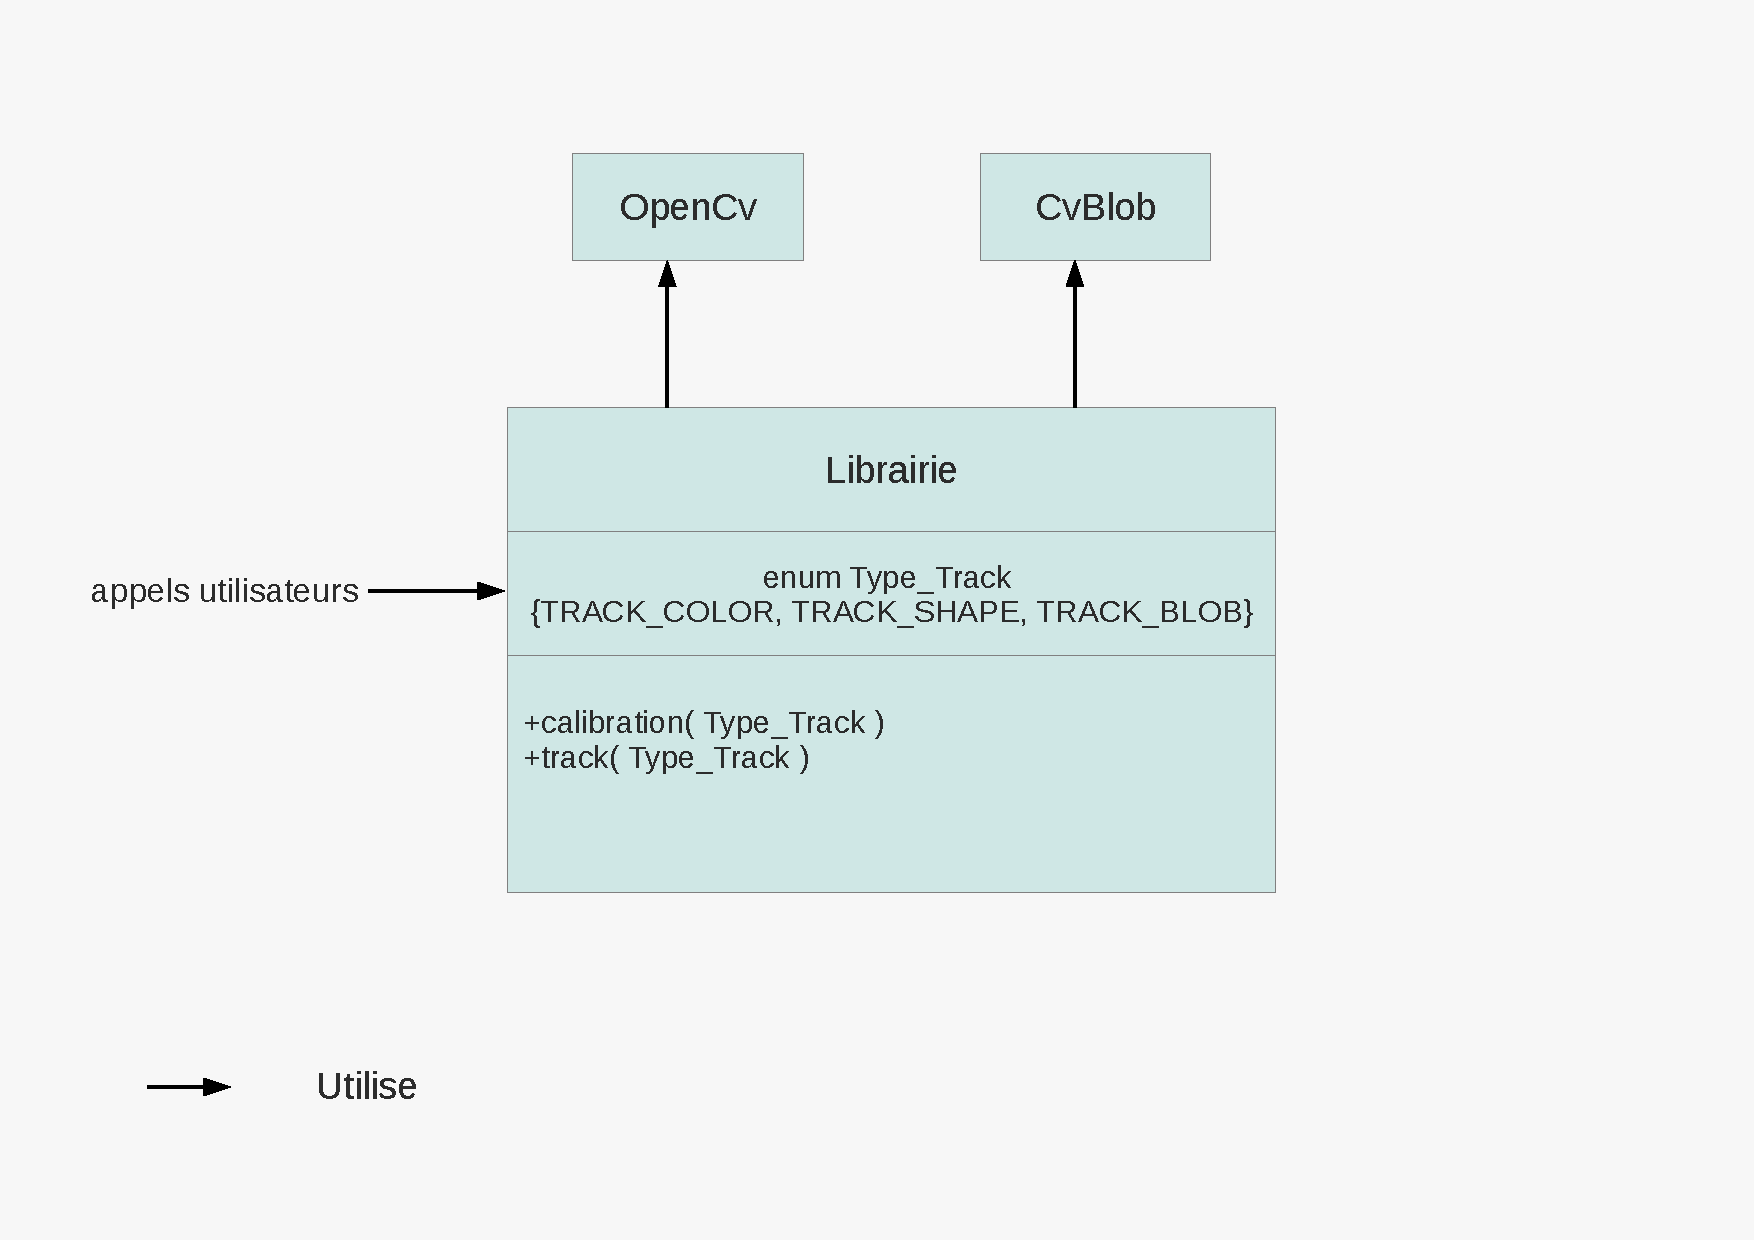
\includegraphics[scale=0.55]{../soutenance/schema-librairie.pdf}\\
						\caption{Architrecture de la bibliothèque}
						\label{Architrecture de la bibliothèque}
					\end{figure}
				\newpage
				\subsubsection{Structure de données}
				\subsubsection{Fonctions}
			\subsection{}
		\section{Application}
	
	\chapter{Résultats}
		\section{Bibliothèque}
		\section{Application}
	
	\chapter{Conclusion}
		\section{Difficultés rencontrées}
		\section{Perspectives}
		\section{Conclusion}
	
	\chapter{Références}
	
	\part{Annexes}
	\appendix
		\chapter{Documentation de la librairie}	
\end{document}
